%% This is file `elsarticle-template-1-num.tex',
%%
%% Copyright 2009 Elsevier Ltd
%%
%% This file is part of the 'Elsarticle Bundle'.
%% ---------------------------------------------
%%
%% It may be distributed under the conditions of the LaTeX Project Public
%% License, either version 1.2 of this license or (at your option) any
%% later version.  The latest version of this license is in
%%    http://www.latex-project.org/lppl.txt
%% and version 1.2 or later is part of all distributions of LaTeX
%% version 1999/12/01 or later.
%%
%% Template article for Elsevier's document class `elsarticle'
%% with numbered style bibliographic references
%%
%% $Id: elsarticle-template-1-num.tex 149 2009-10-08 05:01:15Z rishi $
%% $URL: http://lenova.river-valley.com/svn/elsbst/trunk/elsarticle-template-1-num.tex $
%%
\documentclass[preprint,12pt]{elsarticle}

%% Use the option review to obtain double line spacing
%% \documentclass[preprint,review,12pt]{elsarticle}

%% Use the options 1p,twocolumn; 3p; 3p,twocolumn; 5p; or 5p,twocolumn
%% for a journal layout:
%% \documentclass[final,1p,times]{elsarticle}
%% \documentclass[final,1p,times,twocolumn]{elsarticle}
%% \documentclass[final,3p,times]{elsarticle}
%% \documentclass[final,3p,times,twocolumn]{elsarticle}
%% \documentclass[final,5p,times]{elsarticle}
%% \documentclass[final,5p,times,twocolumn]{elsarticle}

%% The graphicx package provides the includegraphics command.
\usepackage{graphicx}
%% The amssymb package provides various useful mathematical symbols
\usepackage{amssymb}

%% The amsthm package provides extended theorem environments
%% \usepackage{amsthm}

%% The lineno packages adds line numbers. Start line numbering with
%% \begin{linenumbers}, end it with \end{linenumbers}. Or switch it on
%% for the whole article with \linenumbers after \end{frontmatter}.
\usepackage{lineno}

\usepackage{subfigure}
%% Shengyao added the following packages
%\usepackage{outlines}

%% Shengyao added following comments
\interfootnotelinepenalty= 1000

%% Justin added the following packages
\usepackage{amsmath}

%% Boris added the following packages
\usepackage{stmaryrd}

%% natbib.sty is loaded by default. However, natbib options can be
%% provided with \biboptions{...} command. Following options are
%% valid:

%%   round  -  round parentheses are used (default)
%%   square -  square brackets are used   [option]
%%   curly  -  curly braces are used      {option}
%%   angle  -  angle brackets are used    <option>
%%   semicolon  -  multiple citations separated by semi-colon
%%   colon  - same as semicolon, an earlier confusion
%%   comma  -  separated by comma
%%   numbers-  selects numerical citations
%%   super  -  numerical citations as superscripts
%%   sort   -  sorts multiple citations according to order in ref. list
%%   sort&compress   -  like sort, but also compresses numerical citations
%%   compress - compresses without sorting
%%
%% \biboptions{comma,round}

% \biboptions{}

\journal{Journal Name}

\begin{document}

\begin{frontmatter}

%% Title, authors and addresses

\title{Practical Approximation Approaches to Forecasting and Backtesting Initial Margin Requirements}

\author{Justin Chan \footnote{FIS} , Shengyao Zhu \footnote{Nordea} \footnote{, The opinions and views expressed in this paper are those of the author,and do not necessarily represent those of the bank}, Boris Tourtzevitch \footnote{FIS}}

\address{}

\begin{abstract}
As BCBS-IOSCO's introduction of mandatory bilateral initial margin is expected to transform the bilateral OTC market, there has been a great interest in the market to develop a model that can dynamically forecast initial margin for future horizons. The authors proposed practical methods to simulate initial margin requirements, along with validation and historical backtesting approaches, under the context of counterparty credit risk management and regulatory capital calculation. The authors also demonstrated a few testing approaches which are applicable to a broad class of initial margin simulation approaches.

\end{abstract}

\begin{keyword}
Approximation Model \sep BCBS-IOSCO \sep Counterparty Credit Risk \sep internal models method \sep Initial Margin Simulation \sep Margin Reform \sep Regulatory Capital \sep SIMM

\end{keyword}

\end{frontmatter}

%%
%% Start line numbering here if you want
%%

%% main text
\section{Introduction}

Since BCBS-IOSCO's introduction of bilateral initial margin, there has been a great interest in the industry for developing a model that can dynamically forecast initial margin for future time horizons(\cite{anfuso2016sound}, \cite{andersen2016rethinking}). As the introduction of the additional margin requirement is essentially a mechanism to exchange counterparty credit risk with the short term collateral liquidity risk as well as the long term collateral funding cost, an appropriate initial margin simulation model is essential to sound management of credit risk management, capital calculation, as well as funding and liquidity risk management. In this paper, we provide the details of several practical approximation approaches to simulating initial margin, as well as possible validation and backtesting methods and comparison results, with a particular focus on computing counterparty credit risk and regulatory capital calculation.

The paper is organized as follows: Section \ref{sec:background} introduces the background of the margin reform, Section \ref{sec:model} provides the model specifications for simulating initial margin. Sections \ref{s:ExceptionCounting} and \ref{sec:backtesting} demonstrates statistical testing and historical back-testing results for the proposed model by using realistic portfolios and historical market data. Finally, we draw conclusion on section \ref{sec:conclusion}.

\section{Background} \label{sec:background}

\subsection{Margin Reform and Requirements for Non-centrally Cleared Derivatives}

As part of the commitment from Group of 20 (G20) to stabilize and protect the financial system following the crisis in 2008, the Basel Committee on Banking Supervision (BCBS) and the International Organization of Securities Commissions (IOSCO) created the Working Group on Margining Requirements (WGMR) to establish global requirements for margining of non-cleared OTC derivatives.

In March 2015, the WGMR published a final policy framework for non-centrally cleared derivatives. The final framework imposes wide-ranging changes such as the universal exchange of variation margin (VM) and two-way initial margin (IM) [1]. In section 3.1 of the requirement, it requires that the initial margin should ``reflect an extreme but plausible estimate of an increase in the value of the instrument that is consistent with a one-tailed 99 percent confidence interval over a 10-day horizon'', and ``the required amount of initial margin may be calculated by reference to either (i) a quantitative portfolio margin model or (ii) a standardized margin schedule''. Many banks are expected to take the first approach to calculate required initial margin amount, and a widely used industry-standard model is the Standard Initial Margin Model (SIMM) model proposed by ISDA. The focus of this paper is to forward simulate the margin requirement of (i), as the margin requirement of (ii) is specified by a lookup table and is straightforward.

The target of ISDA SIMM model is to provide a common initial margin (IM) methodology that can be used by market participants globally. The model was developed by a work stream initiated by ISDA and major participating banks. For the sake of speed and lower implementation costs, the ISDA SIMM model is designed as a delta-gamma sensitivity-based approach, and the model parameters are to be re-calibrated no less than annually. The details of the ISDA SIMM model can be found in the methodology paper(\cite{isda_im_method_2016}, \cite{isda_im_cacl_process_2016}).

\subsection{Challenges to Forecasting Initial Margin in Credit Exposure Framework}

In typical simulation-based counterparty credit exposure framework, both the aged portfolio value and the collateral value are simulated jointly until the portfolio maturity. This is typically done for either regulatory counterparty credit risk (CCR) capital calculation(\cite{Basel2011BaselIII}) or bank internal CCR management(\cite{gregory2012Counterparty}). Within these frameworks, the initial margin needs to be foreward simulated. As the initial margin is not a constant value for a given portfolio, but will instead vary over time and depend on market movements and trades aging, banks need a model that can forecast it dynamically over future time horizons within the credit exposure calculation framework.

If a bank chooses to use the ISDA SIMM model to calculate initial margin, a natural option would be to brute force replicate the ISDA SIMM model at each simulation horizon and scenario. However, this solution has a serious practical challenge: it requires calculating sensitivities for a large number of risk factors at each horizon and scenario, as sensitivities are the key input to the ISDA SIMM model. While calculating large amount of sensitivities for each horizon and scenario is not unattainable\footnote{possible approaches to generating large amount of sensitivities efficiently include Adjoint Algorithmic Differentiation (AAD) or adopting the GPU technology(\cite{risk2015AADGPU}). Hoever, these approaches are not always immediately available in many production systems.}, getting around the computational performance challenge is not trivial for many production implementations. Instead, an approximation method can be quite attractive, in this document, we describe and compare approximation methods that can be used in production CCR framework, as well as possible validation approaches.

\section{The Simulation Model} \label{sec:model}

In this section we describe three possible approximation methods to forward simulating initial margins, viewed essentially as a problem to estimating forward portfolio Value-at-Risk(VaR). Section \ref{s:GeneralFramework} introduces the general notation and approach to all three methods. Section \ref{s:SimpleVaR} describes a simple approach that estimates portfolio VaR from simulated portfolio changes. Section \ref{s:NadarayaWatsonRegression} describes a non-parametric regression approach that estimates conditional portfolio distribution via a Nadaraya-Watson kernel. Section \ref{s:ParametricRegression} describes a parametric regression approach that estimates conditional portfolio distribution via least-squares. Section \ref{s:OpeningBalanceAndHaircut} provides further adjustments.

\subsection{General Framework}\label{s:GeneralFramework}
Given a portfolio, let $V(t)$  be its value as of time $t$. In a practical Monte Carlo simulation for computing counterparty credit risk, we assume that we have forward simulated portfolio values for a discrete set of scenario paths. More specifically, let $V_{j}(t_{i})$ be the simulated portfolio value on simulation horizon $t_{i}$ and scenario path $j$, where $i=1,...,H$ is the horizon index and $j=1,...,N$ is the scenario index. Note by definition $V_{j}(t_{i})$ excludes the value of cash payments on $t_{i}$. Further, let $C_{j}(t_{i},t_{i+1})$ be the net cash of the portfolio over time span $(t_{i},t_{i+1}]$ on $j$th scenario. We define the cash-adjusted portfolio porfit-and-loss (PnL) $\Delta\bar{V_{j}}(t_{i},t_{i+1})$ as
\begin{equation}
\Delta\bar{V_{j}}(t_{i},t_{i+1})\equiv V_{j}(t_{i+1})-V_{j}(t_{i})+C_{j}(t_{i},t_{i+1}).
\end{equation}
The general approach is to estimate the quantile, $\textrm{Quantile}_{j}^{(q)}(t_{i},t_{i+1})$, of the portfolio value distribution from $V_{j}(t_{i})$ and $\Delta\bar{V}_{j}(t_{i},t_{i+1})$ conditional on realized events on $t \le t_i$. Once obtained, the intent is to approximate initial margin as a $99\%$, 10-business day VaR from the collateral poster's perspective. More specifically, 
\begin{equation}\label{eq:unadjustedReceivedIM}
\textrm{IM}_{j}^{\textrm{received}}(t_{i})=\textrm{Quantile}_{j}^{(99\%)}(t_{i},t_{i}+d)
\end{equation}
is the \emph{unadjusted} received initial margin, and 
\begin{equation}\label{eq:unadjustedPostedIM}
\textrm{IM}_{j}^{\textrm{posted}}(t_{i})=-\textrm{Quantile}_{j}^{(1\%)}(t_{i},t_{i}+d).
\end{equation}
is the \emph{unadjusted} posted initial margin. Further adjustments, such as reconciling with the collateral opening balance, and application of a conservative modelling haircut, are discussed in Section \ref{s:OpeningBalanceAndHaircut}. 

The Simple VaR method in Section \ref{s:SimpleVaR} directly estimates $\textrm{Quantile}_{j}^{(q)}(t_{i},t_{i+1})$, but both non-parametric and parametric regression methods in Sections \ref{s:NadarayaWatsonRegression} and \ref{s:ParametricRegression} estimate the quantiles by first estimating the conditional portfolio moments. More specifically, we look to estimate the $k$th moment $M_{ij}^{(k)}$ of the cash-adjusted portfolio PnL on $i$th horizon and $j$th scenario conditional on information at time $t_i$ along $j$th scenario path as
\begin{equation}\label{eq:momentDefinition}
M_{ij}^{(k)}\equiv\mathbb{E}\left[\left(\Delta\bar{V}_{j}(t_{i},t_{i+1})\right)^{k}|\mathcal{F}_{j}(t_{i})\right].
\end{equation}
Once we can obtain $M_{ij}^{(k)}$, we may infer $\textrm{Quantile}_{j}^{(q)}(t_{i},t_{i+1})$ from these conditional moments. For example, conditional on $j$th simulation path at time $t_i$, assuming that the portfolio distribution is locally normal-distributed, we can find that
\begin{equation}\label{eq:localNormalityQuantile}
\textrm{Quantile}_{j}^{(q)}(t_{i},t_{i+1})=M_{ij}^{(1)}+\sigma_{j}(t_{i},t_{i+1})\Phi^{-1}\left(q\right),
\end{equation}
 \begin{equation}
\sigma_{j}(t_{i},t_{i+1})=\sqrt{M_{ij}^{(2)}-\left(M_{ij}^{(1)}\right)^{2}},
\end{equation}
where $\Phi\left(.\right)$ is the cumulative distribution function of the normal distribution. This \emph{local normality} assumption may be relaxed; possible extension is described in Section \ref{s:CornishFisherExpansion}.

\subsection{Simple VaR}\label{s:SimpleVaR}
The simple VaR approach directly estimates the initial margin by using the sample quantile of $\Delta\bar{V}_{j}(t_{i},t_{i+1})$. More specifically, the unadjusted received initial margin
\begin{equation}
\textrm{IM}_{j}^{\textrm{received}}(t_{i})=\textrm{Quantile}^{(99\%)}\left[\Delta\bar{V}_{j'}(t_{i},t_{i}+10)\right]_{j'=1}^{j'=N},
\end{equation}
 where $\textrm{Quantile}^{(99\%)}\left[.\right]$ is the $\left((99\%)N+1\right)$th element of $\Delta\bar{V}_{j'}(t_{i},t_{i}+10)$ when it's ranked in descending order. The unadjusted posted initial margin can be obtained analogously. Note that under this method, given a simulation horizon $t_i$, simulated initial margin is the same across all scenarios.

\subsection{Non-parametric Regression and the Nadaraya-Watson Kernel}\label{s:NadarayaWatsonRegression}
Another possible approximation method is via a non-parametric regression. Assuming that portfolio value is a good explanatory factor for the state of the portfolio dynamics, to estimate the conditional moments in Equation (\ref{eq:momentDefinition}) we attempt to draw a relationship between the moments of portfolio PnL against portfolio value via a Nadaraya-Watson kernel. The use of the Nadaraya-Watson kernel for simulating initial margin is proposed in \cite{andersen2016rethinking}. In this paper, we presented additional details, as well as validation results.

\subsubsection{The Nadaraya-Watson Kernel}
Given a kernel bandwidth $h_{ij}$ for a given horizon $i$ and scenario $j$, the moments are estimated as\footnote{The use of cash-adjusted PnL, $\Delta\bar{V}_{j}(t_{i},t_{i+1})$, is to exclude the effect of deterministic change in portfolio value due to cash payment events, which should not factor into VaR estimation. Additionally, as we exclude the effect of cash payments during the initial margin horizon when determining portfolio VaR, this cash amount should not be part of the regressor during regression analysis. Hence, we regress against the cash-adjusted portfolio value $\bar{V}_{j}(t_{i},t_{i+1})$. Similar construct is used in Section \ref{s:ParametricRegression}} 
\begin{equation}\label{eq:NadarayaWatsonMoments}
M_{ij}^{(k)}(X_{ij})=\frac{1}{W_{ij}}\sum_{j'=1}^{N}\mathcal{K}\left(\bar{V}_{j}(t_{i},t_{i+1}),\bar{V}_{j'}(t_{i},t_{i+1}),h_{ij}\right)\left(\Delta\bar{V}_{j}(t_{i},t_{i+1})\right)^{k},
\end{equation}
where $\mathcal{K}\left(x,y,h\right)$ is some regression kernel function, and
\begin{equation}
W_{ij}=\sum_{j'=1}^{N}\mathcal{K}\left(\bar{V}_{j}(t_{i},t_{i+1}),\bar{V}_{j'}(t_{i},t_{i+1}),h_{ij}\right)
\end{equation}
is the normalization factor. 

The kernel function $\mathcal{K}\left(x,y,h\right)=\frac{1}{h}\boldmath{K}\left(\left(x-y\right)/h\right)$, where $\boldmath{K}\left(u\right)$ is a standardized kernel, should satisfy the following relations,
\begin{equation}
\boldmath{K}\left(-u\right)= \boldmath{K}\left(u\right),
\end{equation}
\begin{equation}
\int_{-\infty}^{\infty}\boldmath{K}\left(u\right)du = 1.
\end{equation}

In practice, many types of kernels can be used. Examples are
 the Guassian Kernel,
\begin{equation}
\boldmath{K}_{\textrm{Gaussian}}\left(u\right)=\frac{1}{\sqrt{2\pi}}\exp\left[-\frac{1}{2}u^{2}\right],
\end{equation}
or the Epanechnikov kernel,
\begin{equation}
\boldmath{\boldmath{K}}_{\textrm{Epanechnikov}}\left(u\right)=\frac{3}{4}\left(1-u^{2}\right)\mathbf{1}_{\left\{ |u|\le1\right\} }.
\end{equation}
Both the Gaussian and the Epanechnikov kernels are examples of order-2 kernels\cite{Hansen2017Econometrics}.

To use a regression kernel, a bandwidth $h$ must be selected. Choosing the optimal bandwidth can be an art. In practice, we apply the Silverman's Rule of Thumb\citep{Hansen2017Econometrics,Silverman1986Density}. Given a horizon index $i$, define the unconditional standard deviation $Q_{i}$ of the portfolio value as
\begin{equation}
Q_{i}=\left\{ \sum_{j=1}^{N}\left(\bar{V}_{j}(t_{i},t_{i+1})\right)^{2}-\left(\sum_{j=1}^{N}\bar{V}_{j}(t_{i},t_{i+1})\right)^{2}\right\} ^{1/2},
\end{equation}
where
\begin{equation}\label{eq:cashAdjustedPV}
\bar{V}_{j}(t_{i},t_{i+1})\equiv V_{j}(t_{i})-C_{j}(t_{i},t_{i+1}).
\end{equation}
is the portfolio value adjusted for upcoming cash $\bar{V_{j}}(t_{i},t_{i+1})$.
Then, we choose the kernel bandwidth as\footnote{in general, selecting bandwidth for conditional nonparametric regression can be tricky, and statistical techniques such as cross validation\citep{Hansen2017Econometrics} is unlikely to be fast enough in our context, where we have to perform regression for large number of horizons and scenarios. In practice, the Silverman's Rule of Thumb appears to be practical. In practice it is possible to use the conditional standard deviation estimated at previous time step $t_{i-1}$ instead of the unconditional standard deviation $Q_{i}$. However, this introduces additional path dependency. For simplicity, we opt to use the unconditional standard deviation instead.}
\begin{equation}
h_{ij}=\mathbf{C}Q_{i}N^{-1/\left(2d+1\right)}
\end{equation}
where $N$ is the number of scenarios. $d$ is the order of the regression kernel used. More specifically, since both Gaussian or Epanechnikov kernels are of order-$2$, $d=2$. The default value of the constant $\mathbf{C}$ is $2.34$.

\subsubsection{Performance and Thinning}
With a Nadaraya-Watson kernel, in principle we need to apply Equation (\ref{eq:NadarayaWatsonMoments}) for each simulation horizon and scenario, and this many regression computations can present a performance challenge in practice, especially when banks supporting derivatives trading and intra-day risk management may require collateral simulation to be completed on a near-real time basis. We present a simple approach where we only apply Equation (\ref{eq:NadarayaWatsonMoments}) on a subset of scenarios for each simulation horizon.

Choose an integer $M$ such that $M\le N$. Below is a thinning procedure where we will choose to only perform Equation (\ref{eq:NadarayaWatsonMoments}) for $M+1$ out of $N$ scenarios:
\begin{enumerate}
\item For each horizon $i$, sort the portfolio value $\bar{V}_{j}(t_{i},t_{i+1})$ in ascending order. This means there exists an index mapping $J(j)$ such that $\bar{V}_{J(1)}<\bar{V}_{J(2)}<...<\bar{V}_{J(N)}$. 
\item Let $G\equiv\lceil\frac{N}{M}\rceil$, where $\lceil.\rceil$ is the ceiling function. 
\item Perform Equation (\ref{eq:NadarayaWatsonMoments}) for scenarios with indices $j$ such that
\begin{equation}
j\in\left\{ J(mG)|mG<N,m=1,2,3,...\right\} \cup\left\{ J(1),J(N)\right\}.
\end{equation}
\item Based on Step 3, we can create a linearly iterpolated curve with $(M+1)$ grid points, whose abscissa is the portfolio value $\bar{V}_{j}(t_{i},t_{i+1})$ and ordinate the simulated initial margin value $\textrm{IM}_{j}(t_{i})$.
\item For the rest of $(N-M-1)$ scenarios, instead of performing full regression analysis to obtain the simulated initial margin value, the initial margin value will be interpolated off the curve created in Step 4.
\end{enumerate}
Empirically, it appears that it is typically sufficient to choose $M$ such that $M/N$ is around $10\%$ to $20\%$. Comparison results can be found in Section \ref{s:PvAndVaR}.

\subsection{Parametric Regression and the Least-Squares Regression}\label{s:ParametricRegression}
Inspired by American Monte Carlo approaches(\citep{longstaffSchwartz2001AMC}), another approach to estimating the conditional moments in Equation (\ref{eq:momentDefinition}) is via the least-squared regression. Similar ideas are also proposed in \citep{anfuso2016sound}. More precisely, assume we are able to write
\begin{equation}\label{eq:regressionAssumption}
M_{ij}^{(k)}(X_{ij})=\mathbb{E}\left[\left(\Delta\bar{V}_{j}(t_{i},t_{i+1})\right)^{k}|\mathcal{F}_{j}(t_{i})\right]=\sum_{l=1}^{L}\beta_{i,l}^{(k)}\psi_{l}^{(k)}(X_{ij}),
\end{equation}
where $X_{ij}$ is the risk factor state on $i$th horizon and $j$th scenario. $\psi_{l}^{(k)}(X_{ij})$, $l=1,...,L$ is a set of basis functions that needs to be chosen such that a suitable linear combination of these basis functions well describes the relationship between portfolio value and its future PnL. Note that while in general the set of basis functions need not be the same for each moment, for simplicity we choose the same set for each moment $k$. In practice, we choose it to be the monomials of cash-adjusted portfolio value as of time $t_{i}$

\begin{equation}
\psi_{l}^{(k)}(X_{ij})=\left(\bar{V}_{j}(t_{i},t_{i+1})\right)^{l},
\end{equation}
where $\bar{V}_{j}(t_{i},t_{i+1})$ is defined in Equation (\ref{eq:cashAdjustedPV}). The positive integer $L$ is the number of basis functions. The basis function coefficients $\beta_{i,l}^{(k)}$ are to be calibrated via least-squares. Once calibrated, given portfolio values, we can determine the moments of the portfolio distribution.

Multiplying both sides of Equation (\ref{eq:regressionAssumption}) of by $\psi_{l'}^{(k)}(X_{ij})$ and taking conditional expectation yields
\begin{equation}\label{eq:regressionEquation}
\mathbb{E}\left[\psi_{l'}^{(k)}(X_{ij})\left(\Delta\bar{V}_{j}(t_{i},t_{i+1})\right)^{k}|\mathcal{F}_{j}(t_{i})\right]=\sum_{l=1}^{L}\beta_{i,l}^{(k)}\mathbb{E}\left[\psi_{l}^{(k)}(X_{ij})\psi_{l'}^{(k)}(X_{ij})|\mathcal{F}_{j}(t_{i})\right].
\end{equation}
 Alternately, in matrix notations, for convenience define
\begin{equation}\label{eq:alphaDefinition}
\boldsymbol{\alpha}_{i}^{(k)}=\alpha_{i,l}^{(k)}\equiv\mathbb{E}\left[\psi_{l'}^{(k)}(X_{ij})\left(\Delta\bar{V}_{j}(t_{i},t_{i+1})\right)^{k}|\mathcal{F}_{j}(t_{i})\right],
\end{equation}
\begin{equation}\label{eq:BDefinition}
\boldsymbol{B}_{i}^{(k)}=B_{i,ll'}^{(k)}\equiv\mathbb{E}\left[\psi_{l}^{(k)}(X_{ij})\psi_{l'}^{(k)}(X_{ij})|\mathcal{F}_{j}(t_{i})\right],
\end{equation} 
\begin{equation}\label{eq:betaDefinition}
\boldsymbol{\beta}_{i}^{(k)}\equiv\beta_{i,l}^{(k)}.
\end{equation} 
Note that in Equations (\ref{eq:alphaDefinition} - \ref{eq:betaDefinition}), we have suppressed the indices $l$ and $l'$ for the boldfaced vector notations. More specifically, given a particular horizon index $i$ and moment index $k$, the boldfaced $\boldsymbol{\alpha}_{i}^{(k)}$ and $\boldsymbol{\beta}_{i}^{(k)}$ are vectors of length $L$, and the boldfaced $\boldsymbol{B}_{i}^{(k)}$ is a matrix of size $L\times L$. In this matrix notation, Equation (\ref{eq:regressionEquation}) becomes
\begin{equation}
\boldsymbol{\alpha}_{i}^{(k)}=\boldsymbol{B}_{i}^{(k)}\centerdot\boldsymbol{\beta}_{i}^{(k)}.
\end{equation}
With $j=1,...,N$ realized Monte Carlo scenarios, we can estimate elements of $\boldsymbol{\alpha}_{i}^{(k)}$ and $\boldsymbol{B}_{i}^{(k)}$ as
\begin{equation}\label{eq:RegressionInnerProduct}
\alpha_{i,l}^{(k)}=\frac{1}{N}\sum_{j=1}^{N}\psi_{l}^{(k)}(X_{ij})\left(\Delta\bar{V}_{j}(t_{i},t_{i+1})\right)^{k},
\end{equation}
\begin{equation} \label{eq:RegressionBasisNormMatrix}
B_{i,ll'}^{(k)}=\frac{1}{N}\sum_{j=1}^{N}\psi_{l'}^{(k)}(X_{ij})\psi_{l}^{(k)}(X_{ij}).
\end{equation}
Then, after obtaining all elements of $\boldsymbol{\alpha}_{i}^{(k)}$ and $\boldsymbol{B}_{i}^{(k)}$, the basis function coefficients $\boldsymbol{\beta}_{i}^{(k)}$ may be obtained via
\begin{equation}
\boldsymbol{\beta}_{i}^{(k)}=\left(\boldsymbol{B}_{i}^{(k)}\right)^{-1}\centerdot\boldsymbol{\alpha}_{i}^{(k)}.
\end{equation}
Repeat this exercise for every horizon $i$, and we may obtain an estimate for the moments $M_{ij}^{(k)}$ for each $j$th scenario. Note that the least-squares regression is performed once across all scenarios for each horizon.
 
\subsection{Opening Balance and Haircut} \label{s:OpeningBalanceAndHaircut}

The initial margin at $t=0$ requires special care. First, for both non-parametric and parametric approaches from Sections \ref{s:NadarayaWatsonRegression} and \ref{s:ParametricRegression}, we use the cash-adjusted portfolio value introduced in Equation (\ref{eq:cashAdjustedPV}) as the explanatory variable for portfolio PnL quantiles. Specifically, we exclude the upcoming cash payment as that portion of the portfolio value should not be a good explanatory factor of upcoming portfolio PnL distribution. However, a consequence of this feature is that a verbatim implementation of either Sections \ref{s:NadarayaWatsonRegression} or \ref{s:ParametricRegression} unrealistically implies that the unadjusted initial margin values $\textrm{IM}_{j}(0)$ at $t=0$ are scenario-dependent. Instead, for $t=0$, the Simple VaR method from Section \ref{s:SimpleVaR} will be used.

Next, as in practice the initial margin is typically calculated according to the ISDA SIMM model, opening balance of initial margin, denoted $\textrm{IM}_{0}$, is not only known at $t=0$, but the difference between $\textrm{IM}_{0}$ and the $t=0$ unajusted initial margin value, $\textrm{IM}_{j}(0)$, can be material, and We  adjust the simulated initial margin to match the opening balance. The opening balance-adjusted initial margin $\widetilde{\textrm{IM}}_{j}(t_{i})$ is given as
\begin{equation}
\widetilde{\textrm{IM}}_{j}(t_{i})=\left(\frac{\textrm{IM}_{0}}{\textrm{IM}_{j}(t_{0})}\right)\textrm{IM}_{j}(t_{i}).
\end{equation} 

More sophisticated fitting of the initial margin profile has been proposed(\cite{anfuso2016sound}), but the multiplier is adopted for simplicity. Further, as there can be a significant amount of model risk in the approximation methods, in the context of credit risk management and regulatory capital calculation, we introduce an optional model haircut $\mathcal{H}$ to the simulated initial margin. 

\begin{eqnarray}
\widehat{\textrm{IM}}_{j}(t)=\begin{cases}
\textrm{IM}_{0}, & t=0\\
\left(1-\mathcal{H}\right)\widetilde{\textrm{IM}}_{j}(t) & t>0.
\end{cases}
\end{eqnarray} 

In general, under such context, underestimating the amount of initial leads to a more conservative estimate of credit exposure. Such an assumption may not be as suitable in other context, such as managing collateral funding or liquidity risks.
 
\subsection{Cornish-Fisher Expansion}\label{s:CornishFisherExpansion}
It is possible to extend beyond the local normality assumption in Equation (\ref{eq:localNormalityQuantile}). For example, by estimating the first four moments $M_{ij}^{(1)}$, $M_{ij}^{(2)}$, $M_{ij}^{(3)}$ and $M_{ij}^{(4)}$, as well as the conditional skewness $S_{j}(t_{i},t_{i+1})$ and excess kurtosis $K_{j}(t_{i},t_{i+1})$
\begin{equation}
S_{j}(t_{i},t_{i+1})=\frac{1}{\sigma_{j}^{3}(t_{i},t_{i+1})}\left(M_{ij}^{(3)}-3M_{ij}^{(1)}\sigma_{j}^{2}(t_{i},t_{i+1})-\left(M_{ij}^{(1)}\right)^{3}\right),
\end{equation}  
\begin{multline}
K_{j}(t_{i},t_{i+1})=\frac{1}{\sigma_{j}^{4} (t_{i},t_{i+1})}\times \\
\left(M_{ij}^{(4)}-4M_{ij}^{(1)}M_{ij}^{(3)}+6\left(M_{ij}^{(1)}\right)^{2}\sigma_{j}^{2}(t_{i},t_{i+1})+3\left(M_{ij}^{(1)}\right)^{4}\right) -3.
\end{multline}  

we may utilize the Cornish-Fisher expansion(\citep{cornishFisher1960}) to estimate the portfolio PnL quantile
\begin{equation}
\textrm{Quantile}_{j}^{(q)}(t_{i},t_{i+1})=M_{ij}^{(1)}+\sigma_{j}(t_{i},t_{i+1})w_{ij}(z),
\end{equation}
where $z=\Phi^{-1}\left(q\right)$, and 
\begin{equation}
w_{ij}(z)=z+\left[S_{j}(t_{i},t_{i+1})h_{1}(z)\right]+\left[K_{j}(t_{i},t_{i+1})h_{2}(z)+S_{j}^{2}(t_{i},t_{i+1})h_{11}(z)\right],
\end{equation}
\begin{equation}
h_{1}(z)=\frac{1}{6}\left(z^{2}-1\right),
\end{equation}
\begin{equation}
h_{2}(z)=\frac{1}{24}\left(z^{3}-3z\right),
\end{equation}
\begin{equation}
h_{11}(z)=-\frac{1}{36}\left(2z^{3}-5z\right).
\end{equation}

As the local normality assumption typically underestimates the portfolio VaR and initial margin, under the context of credit risk management and regulatory capital calculation, we continue to use the local normality assumption. However, the Cornish-Fisher may be more suitable in other contexts, such as funding and liquidity management.

\subsection{Testing approach}

In the following sections, we will discuss how to test the proposed models presented in this section. There are two category of testing approaches proposed in this paper. The first is to assess the appropriateness of its in-simulation consistency. Essentially, our approximation models forecasting future IM values by attempting to estimate forward VaR values from simulated PnLs and simulated portfolio values. This is discussed in Section \ref{s:ExceptionCounting}. The second is to assess the appropriateness of our simulated IM distribution with respect to its historical distribution. This historical backtesting assessment is elaborated in Section \ref{sec:backtesting}.


\section{Exception Counting and Validation Results}\label{s:ExceptionCounting}

This section will discuss the certain statistical features of the estimated initial margin number, such as its exceptiong counting statistics within the simulation. Section \ref{s:theBenchmarkPortfolio} outlines the benchmark portfolio we use to perform our testings. Section \ref{s:PvAndVaR} explores the relationship between simulated portfolio value and its regression-based VaR. Section \ref{s:ExceptionCounting} describes our exception counting schemes and results.

\subsection{The Benchmark Portfolio}\label{s:theBenchmarkPortfolio}

All tests presented below are based on a benchmark portfolio coming from the real life portfolio that subject to IM regulation, the portfolio contain more than 100 trades and most of them are interest rate swap and interest rate swaptions as well as some cross currency swap. The currencies are dominated mainly by EUR,USD and GBP. The remaining maturities of the portfolio are well distributed between 1 Year and 20 Year horizon, the average remaining maturity of the portfolio is 5 Year. In the test, it is assumed that the portfolio will keep same remaining maturity and same moneyness over the test period.

\subsection{Relationship Between Portfolio Value and VaR}\label{s:PvAndVaR}

For any of the simulation methods proposed in Section \ref{sec:model}, the objective is to infer the scenario-wise initial margin(or VaR) from simulated cash-adjusted portfolio value and simulated PnLs. Hence, one preliminary test is to examine the relationship between the simulated unadjusted initial margin and cash-adjusted portfolio value and PnLs. Figure \ref{fig:PVvsPnL} shows the comparison between the simulated unadjusted initial margin against the scatter plot of cash-adjusted PV vs PnL at the one year simulation horizon for the benchmark portfolio, across the three methods proposed in Section \ref{sec:model}. Intuitively, we expect the unadjusted initial margin to act as an envelope to the cash-adjusted portfolio value vs PnL scatter plot, such that only a small number of simulated cash-adjusted PnLs to exceed it. By construction the unadjusted initial margin produced by Simple VaR method of Section \ref{s:SimpleVaR} is invariant with respect to simulated cash-adjusted portfolio value. Both the Nadaraya-Watson kernel method of Section \ref{s:NadarayaWatsonRegression} and the least-squares parametric approach of Section \ref{s:ParametricRegression} appear to perform respectably, but as the least-squares approach is constrained by the parametric form imposed, appears to be less flexible.

\begin{figure}[h] 
\hfill
\subfigure[Simple VaR]{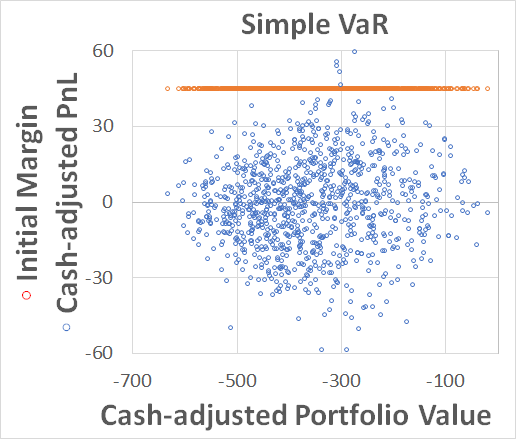
\includegraphics[width=.32\linewidth]{PVvsPnLSimpleVaR.png}}
\hfill
\subfigure[Nadaraya-Watson]{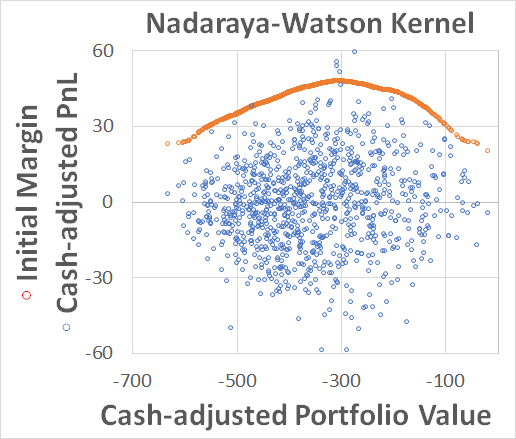
\includegraphics[width=.32\linewidth]{PVvsPnLNadarayaWatson.png}}
\hfill
\subfigure[Least-Squares]{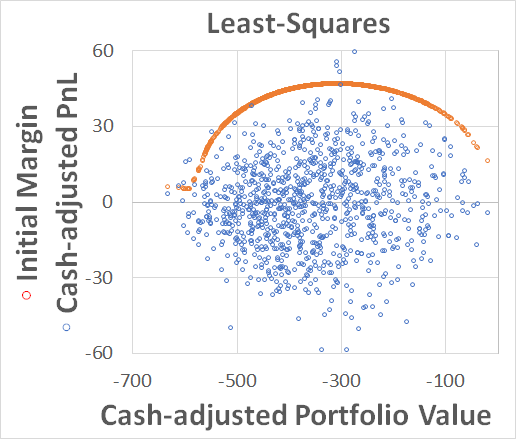
\includegraphics[width=.32\linewidth]{PVvsPnLParametricRegression.png}}
\hfill
\caption{A comparison of scatter plots of portfolio value vs simulated initial margin and PnL for initial margin models. The simulation horizon is 1-yr, with 1000 simulated scenarios. All figures in millions.}
\label{fig:PVvsPnL}
\end{figure}

As discussed in Section \ref{s:NadarayaWatsonRegression}, a challenge of employing the non-parametric kernel approach is that performance can be a challenge. In such instances, thinning provides a practical approach to speed up the calculation. A good demonstration of the comparison of accuracy with the introduction of thinning can also be seen from the scatter plots. Figure \ref{fig:EffectOfThinning} demonstrates this. In the figure, we compare the results where we perform kernel regression for each scenario, against the results where we perform kernel regression for only 50 out of 1000 scenarios.  We see that the results change little.

\begin{figure}[h] 
\hfill
\subfigure[Nadaraya-Watson Kernel, without thinning effect]{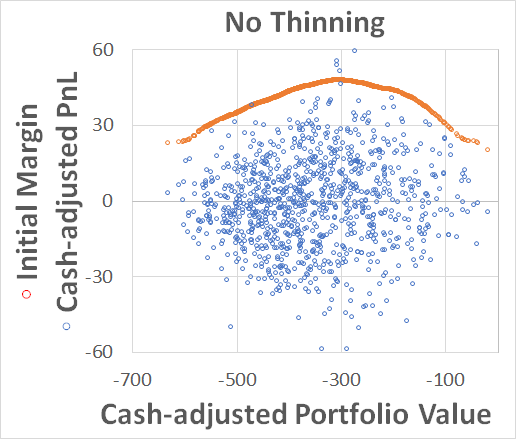
\includegraphics[width=.48\linewidth]{PVvsPnLNadarayaWatsonNoThinning.png}}
\hfill
\subfigure[Nadaraya-Watson Kernel, with only 5\% of scenarios]{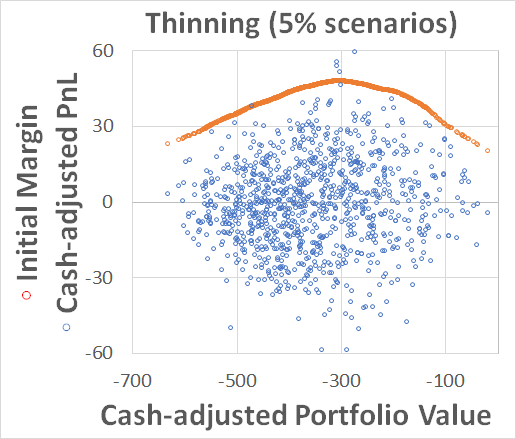
\includegraphics[width=.48\linewidth]{PVvsPnLNadarayaWatsonThinning.png}}
\hfill
\caption{A comparison between the simulation results via the Nadaraya-Watson kernel, with or without thinning. The left graph shows the result where we calculate the unadjusted initial margin for each of the 1000 scenarios. The right only for 50 of the 1000 scenarios, with the rest by interpolation.}
\label{fig:EffectOfThinning}
\end{figure}

\subsection{Exception Counting Schemes}

Inspired by market risk management practices(\citep{Basel1996VaRBacktesting}), One of the simplest ways of validating an initial margin model, focused specifically on the unadjusted initial margins defined in Equations (\ref{eq:unadjustedReceivedIM}) and (\ref{eq:unadjustedPostedIM}), is via \emph{exception counting}. The scheme described below focuses specifically on received initial margin, although posted initial margin can be validated analogously. Concretely, an \emph{exception} occurs when $I_{ij}=1$, where
\begin{eqnarray}
I_{ij}=\begin{cases}
1, & \Delta\bar{V_{j}}(t_{i},t_{i}+d) > \textrm{Quantile}_{j}^{(99\%)}(t_{i},t_{i}+d)\\
0, & \Delta\bar{V_{j}}(t_{i},t_{i}+d) \leq \textrm{Quantile}_{j}^{(99\%)}(t_{i},t_{i}+d).
\end{cases}
\end{eqnarray}
If the Monte Carlo simulation and the initial margin simulation are self-consistent, then the statistics of $I_{ij}$ should have certain patterns. For simplicity, we assume that the initial margin horizons do not overlap, or that $t_{i}+d \leq t_{i+1} \, \forall \, i=1,...,N-1$. There are at least two possible testing schemes. The first is to count exception \emph{across scenarios}, where for any horizon index $i$, the realized average exception rate $r_i$ should be roughly
\begin{equation}
r_i \equiv \frac{1}{N}\sum_{j=1}^{N}I_{ij}\approx 1\%.
\end{equation}
Further, with confidence level $p$, the average exception rate $r_i$ should fall within the confidence interval
\begin{equation}
\left[\frac{B^{-1}(N,1\%,1-p)}{N},\frac{B^{-1}(N,1\%,p)}{N}\right],
\end{equation}
where $B^{-1}(N,p,x)$ is the inverse cumulative distribution function of the binomial distribution with $N$ trials, success probability $p$ for each trial, at quantile level $x$. 

Figure \ref{fig:ExceptionAcrossScenarios} demonstrates the results of simulated exception rates of our benchmark portfolio, using both the Nadaraya-Watson non-parametric kernel of Section \ref{s:NadarayaWatsonRegression} and the least-squares parametric regression of Section \ref{s:ParametricRegression}. The Monte-Carlo simulation runs for $N=5000$ scenarios for 5-years, and we compare the simulated exception rates against the expected exception rate of $1\%$, as well as the $95\%$ confidence interval. While the Nadaraya-Watson kernel appears to be more stable over time, both methods display the same tendency that the exception rate is slightly higher than ideally expected. One source for this tendency is due to the local normality assumption, which typically leads to an underestimation of the initial margin. The local normality assumption may be improved, for example, by using the Cornish-Fisher expansion discussed in Section \ref{s:CornishFisherExpansion} instead. However, in the context of calculating credit exposure, an underestimation of initial margin can generally be tolerated as it leads to a conservative exposure estimate. Note that, by comparison, the Simple VaR method of Section \ref{s:SimpleVaR} is a special case where by construction, the exception rate is always $1\%$ for all horizons.

\begin{figure}[h] 
\hfill
\subfigure[Nadaraya-Watson Kernel]{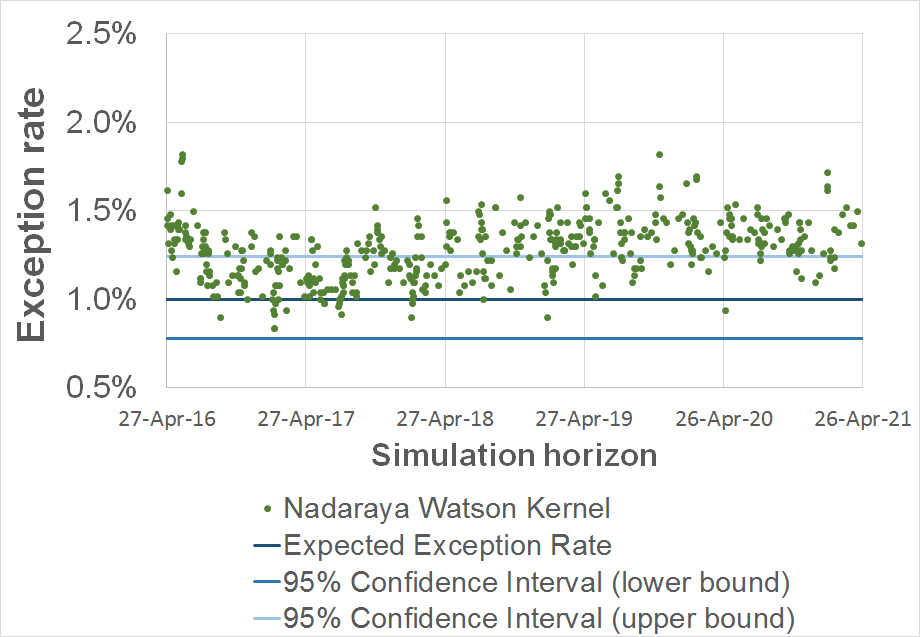
\includegraphics[width=.48\linewidth]{ExceptionAcrossScenarios_NadarayaWatson.png}}
\hfill
\subfigure[Least-Squares Regression]{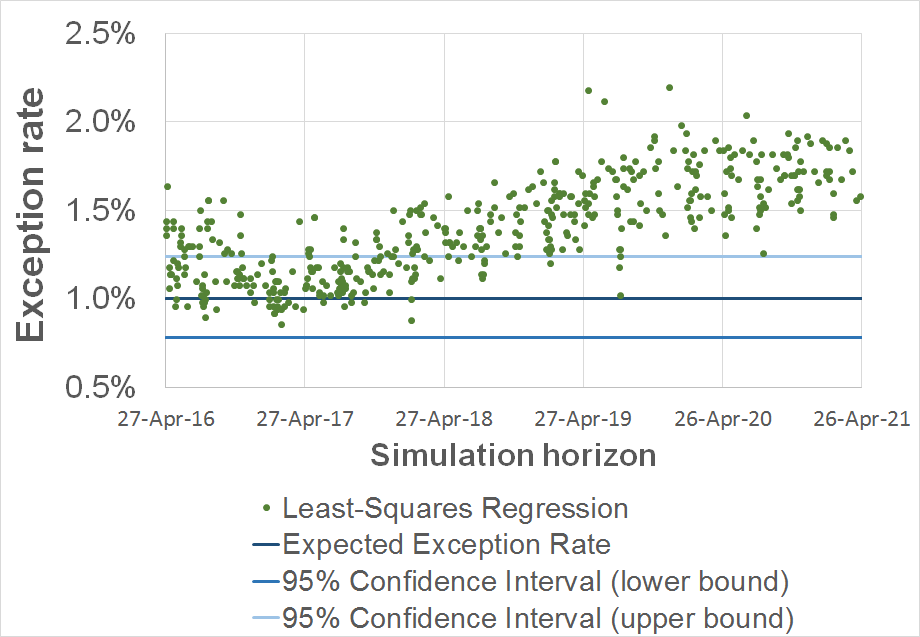
\includegraphics[width=.48\linewidth]{ExceptionAcrossScenarios_ParametricRegression.png}}
\hfill
\caption{A comparison of exception rate across scenarios for initial margin models}
\label{fig:ExceptionAcrossScenarios}
\end{figure}

Another possible exception counting scheme is to count exceptions \emph{through time}. We first collect the exceptions count $E_j$ for scenario $j$ through all horizons
\begin{equation}
E_{j}=\sum_{i=1}^{H}I_{ij}.
\end{equation}
Assuming that exceptions occur randomly with $1\%$ rate, with an ideal simulation method, $E_j$ should be distributed according to a binomial distribution 
\begin{equation}
\mathbb{P}\left(E_{j}=n\right)=b\left(H,1\%,n\right),
\end{equation}
where $b(H,q,n)$ is the probability mass function for a binomial distribution with $H$ trials, success probability $q$ for each trial, at $n$ successes. With $N$ total Monte Carlo scenarios, we can compare the simulated histogram of $E_j$ and compare it with the probability mass function of the binomial distribution.

Figure \ref{fig:ExceptionThroughTime} compares the simulated exception counts $E_j$ for the benchmark portfolio for the three different approaches outlined in Sections (\ref{s:SimpleVaR}-\ref{s:ParametricRegression}). The Monte Carlo simulation runs for $N=5000$ scenarios and $H=585$ non-overlapping two-week periods. The simulated histograms of exception counts are compared against the ideal binomial distribution. The least satisfactory method is the Simple VaR, where the histogram of the simulated exception counts not only differs from that of the ideal binomial distribution, for many Monte Carlo paths, there is actually a tendency to overestimate the initial margins, leading to a lower-than-expected exception counts. This is not preferred in the context of credit exposure simulation, as along these Monte Carlo paths the credit exposures are underestimated. In contrast, the behaviors of the Nadaraya-Watson non-parametric kernel regression and the least-squares parametric regression are more reasonable, with the Nadaraya-Watson kernel behaving slightly better in the example. Both these methods exhibit a tendency to producing higher-than-expected exception counts, which in the context of credit exposure calculation leads to a conservative exposure estimate.

\begin{figure}[h] 
\hfill
\subfigure[Simple VaR]{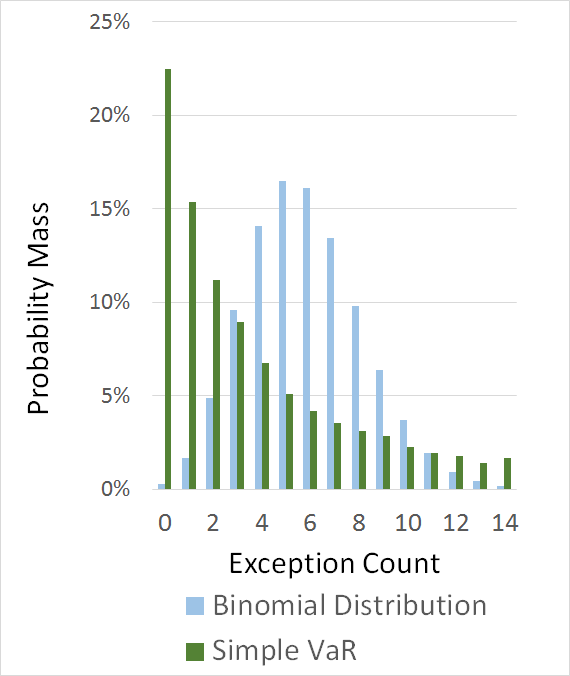
\includegraphics[width=.32\linewidth]{ExceptionThroughTime_SimpleVaR.png}}
\hfill
\subfigure[Nadaraya-Watson]{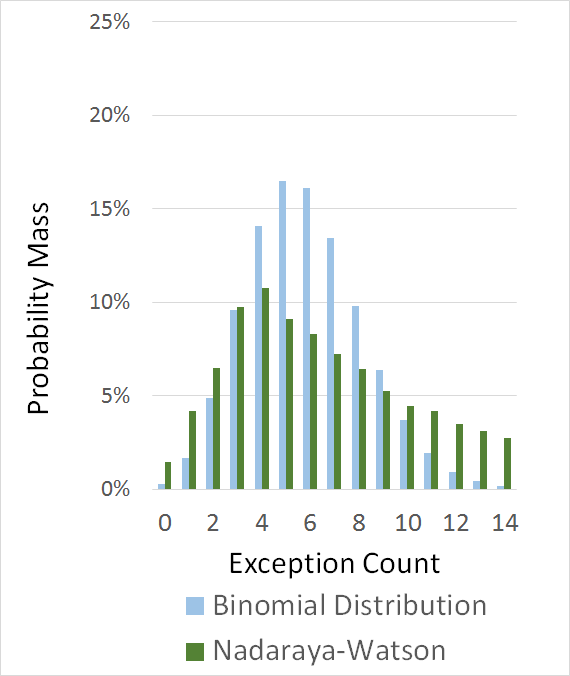
\includegraphics[width=.32\linewidth]{ExceptionThroughTime_NadarayaWatson.png}}
\hfill
\subfigure[Least-Squares]{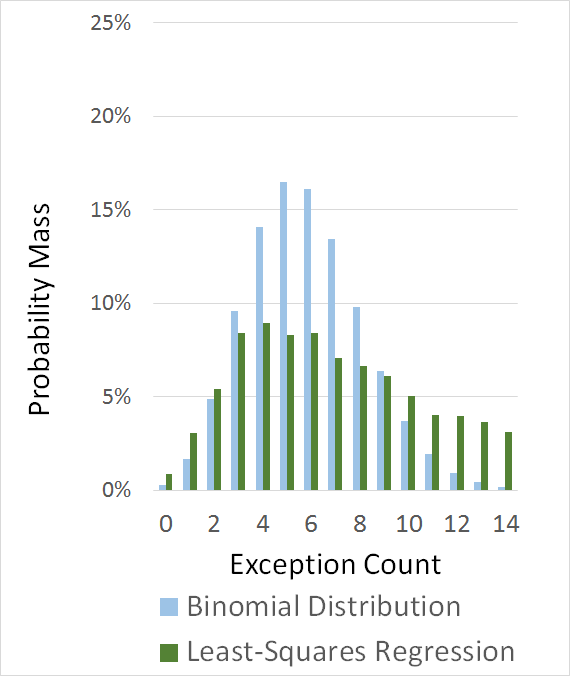
\includegraphics[width=.32\linewidth]{ExceptionThroughTime_ParametricRegression.png}}
\hfill
\caption{A comparison of exception counts through time for initial margin models}
\label{fig:ExceptionThroughTime}
\end{figure}

These exception counting schemes, while simple, can be adopted by many forward-IM or forward-VaR simulation schemes. Further, as the schemes employ existing simulation intermediate results, they adds little to overall simulation effort.

\section{Historical Backtesting of Initial Margin Simulation Models} \label{sec:backtesting}

In Section \ref{s:ExceptionCounting}, we have seen some evidence of in-simulation consistency for the IM distribution as defined by the regression model. Exception counting schemes have come quite handy for that purpose. In this section, we try to estimate how our approximation model compares against historical backtesting. Section \ref{s:backtestingBackground} provides further background and motivation to our backtesting approach. Section \ref{s:dataPrepare} provided some details about data prepared for this testing. Section \ref{sec:spotZeroIMTest} compares the historical spot initial margin value as calculated by the ISDA SIMM model against our approximation model. Section \ref{s:BacktestingProcedure} outlines a backtesting procedure that follows the methodology outlined in \cite{ruiz2014backtesting}. We then presents our backtesting results in Section \ref{s:Results}.

\subsection{Background and Motivation}\label{s:backtestingBackground}

As pointed out by \cite{anfuso2016sound}, depending on the context and the purpose of model usage,  it may or may not be important to have an accurate assessment of the distribution of the simulated IM values against historically realized values. However, under the context of counterparty credit risk management and regulatory capital calculation, it is often deemed sound model risk management to be able to demonstrate appropriate historical backtesting results, either internally or externally to the regulators(\citep{Basel2010Backtesting}). To achieve this, a historical backtesting procedure is introduced to assess the model performance of the proposed model.

Regarding the target of backtesting against which we assess the appropriateness of our IM model, there are at least two viable options: the historical ISDA SIMM values, or the historical 10-day 99\% stressed VaR values. Here we choose to backtest against the ISDA SIMM values, since in practice the market standard is to calculate the collateral amount with respect to the ISDA SIMM model. Also note that the ISDA working group is establishing a backtesting process (\cite{isda_simm_2016}) for ISDA SIMM model which should track the performance of the ISDA SIMM model against the 10 day 99\% stressed VaR.

Further, for illustrative purposes, the backtesting results are done with respect to the Nadaraya-Watson kernel approach of Section \ref{s:NadarayaWatsonRegression}. However, the backtesting approach described here should apply to a broad class of initial margin simulation models. Further, the backtesting results are generated with the model haircut $\mathcal{H}$ introduced in Section \ref{s:OpeningBalanceAndHaircut} set to zero. Within the context of credit risk management and regulatory capital calculation, with the historical backtesting results as a guide, the model haircut $\mathcal{H}$ can be appropriately set to achieve the desired level of conservatism.

\subsection{Data Preparation and Building a Historical SIMM Series}\label{s:dataPrepare}
To support historical backtesting, the first task is to prepare and define the historical data to be used. This broadly includes three aspects:
\begin{itemize}
\item historical market data
\item historical portfolios
\item historical initial margin values
\end{itemize}

For the backtesting study, we select a five year historical backtesting window from 2011 to 2016. We prepare two Scenarios of backtesting data: Real Market Scenario and Hypothetical Market Scenario. We describe their preparation approach and rationales below.

\subsubsection{Real Market Scenario}

This Scenario uses actual historically realized market data for backtesting study. However, what this market data contains needs further specification. As we need to assess the quality of forecasted IM values using our approximatio models against historical IM values, the historical data not only need to include historical market rates(e.g., interest rates, FX rates, etc), but also historical model parameters for the simulation models of the market rates. We use the historical model parameters coming from real-life model which calibrated to the stress period, during the backtesting window for this study.

In addition to historical market data, we also need to prescribe a series of historical portfolios for the backtesting window. We use the benchmark portfolio described in Section \ref{s:theBenchmarkPortfolio}, and with its trade maturities and moneyness adjusted throughout the backtesting window such that the average portfolio maturities and moneyness remain constant through the backtesting window.

The last element of the data preparation is the historical IM values. This presents a practical challenge, as bilateral IM does not come into effect until September 2016 at the earliest. Instead, we take the historical market data and historical benchmark portfolios described above, and compute a series of \emph{would-be} historical portfolio sensitivities and historical IM values  via the ISDA SIMM model through the backtesting window.

\subsubsection{Hypothetical Market Scenario}
Broadly speaking, a successful IM simulation consistent with historical backtesting requires three elements:
\begin{enumerate}
\item A set of forecasting models and their model parameters for the market rates (e.g., interest rates, FX rates, etc) consistent with historical backtesting. 
\item A set of trade valuation models consistent with the calculation of spot IM calculation model (e.g., valuation models used to generate portfolio sensitivities for the ISDA SIMM model).
\item Given a set of market rates paths (historically realized or simulated), an IM forecasting model consistent with the behavior with the spot IM calculation model (e.g., the ISDA SIMM model).
\end{enumerate}

Within our simulation and testing framework, we use same set of valuation models for both forecasting initial margin via approximations, as well as generating portfolio sensitivities for the spot ISDA SIMM calculation and preparation of historical IM values, so element 2 above should not be a significant contributor to our backtesting result. The focus of Section \ref{sec:model} is to define a suitable model for element 3. However, even with a suitable IM forecasting model, the simulated IM values can still be inconsistent with historical backtesting due to poor forecasting of market rates of element 1. Hence, it is important to prepare testing data to be able to separate the effects of element 1 and 3. 

To this end, we prepare a different set of backtesting data separate from the Real Market Scenario above. We fix the market rates simulation model parameter constant throughout the five-year backtesting window, and take the historical market rates at the beginning of the backtesting window (i.e., 2011) as the initial point. We then forward project a series of daily market rates for the entire backtesting window, and use the simulated market rates as substitute for actual historical market data instead. We then take the same series of portfolio as for the Real Market Scenario, and apply the same approach to construct the \emph{would-be} historical ISDA SIMM IM values. 

The objective of creating a Hypothetical Market Scenario\footnote{In fact, we can create multiple versions of Hypothetical Market Scenarios with the same set of model parameters, to further study the statistical properties.} separate from the Real Market Scenario is that a comparison between the backtesting results of the two Scenarios highlights the impact of simulation models used for market rates.

\subsection{Comparing spot Initial Margins by the ISDA SIMM model vs the Approximation Model} \label{sec:spotZeroIMTest}

The simplest historical backtesting is to assess the model performance at $t=0$. More specifically, in this section, we compare the correlation between the spot initial margin calculated by ISDA SIMM model against the spot initial margin calculated by our approximation model without adjustment to the opening balance provided by the ISDA SIMM model. The purpose of this test is to investigate whether the proposed initial margin model can capture the same market dynamic as ISDA SIMM model in a changing market scenario. 

The calculation is performed on daily step over the five year market scenario. The tests are performed for both the Hypothetical Market Scenario and the Real Market Scenario. The results, scatter plots of initial margains by the ISDA SIMM model against the approximation model over the five year window, are summarized in Figure \ref{fig:correlation_plot}.

\begin{figure}[h] 
\hfill
\subfigure[Hypothetical Market Scenario]{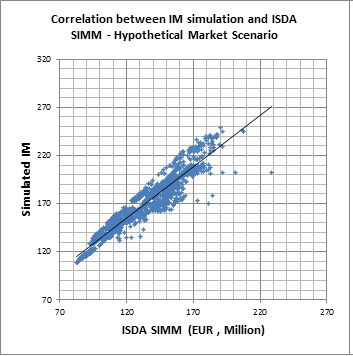
\includegraphics[width=.45\linewidth]{im_test_hypo_scenario.PNG}}
\hfill
\subfigure[Real Market Scenario]{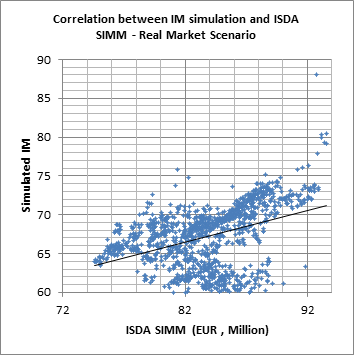
\includegraphics[width=.45\linewidth]{im_test_real_scenario.PNG}}
\hfill
\caption{Correlation between IM with the ISDA SIMM model and the Approximation Model}
\label{fig:correlation_plot}
\end{figure}

The \emph{left part} of Figure \ref{fig:correlation_plot} show the result for the Hypothetical Market Scenario. The result demonstrates a strong positive correlation between the spot IM given by the approximation model and the ISDA SIMM model over time. In this Scenario, the same set of market rates model parameters is used for both generating the historical market rates and simulating the initial margin. It also demonstrates the desired strong correlation between the proposed approximatio model and the ISDA SIMM model for the calculation of the spot initial margin. The same tests have been performed in additional Hypothetical Market Scenarios, and all tests show the same pattern. By all these tests, we conclude the proposed IM simulation model is as sensitive as ISDA SIMM model respect to the market movement. 

As described in Section \ref{sec:model}, the proposed initial margin simulation model takes the simulated portfolio values at the forward time horizon as input, the forecast quality of the initial margin simulation model partially depends on the appropriateness of the market rates simulation models. To demonstrate this, we repeat the above test using the Real Market Scenario, where the market rates simulation models does not have the same dynamics as the historical market rates. As shown by the \emph{right part} of Figure \ref{fig:correlation_plot}, the correlation is not as significant. This study emphasizes the importance of anchoring the spot initial margin to the opening IM balance calculated by the ISDA SIMM model, as  described in section \ref{s:OpeningBalanceAndHaircut}.

\subsection{The Backtesting Procedure}\label{s:BacktestingProcedure}

The next step is to assess the forecasting quality of our approximation model. We describe our backtesting approach in this section, and present our results in Section \ref{s:Results}. We follow the approach of \citep{ruiz2014backtesting}: given a backtesting window $[t_{\textrm{start}}, t_{\textrm{end}}]$ (i.e., 2011-2016) and a forecasting horizon $\Delta_f$ (e.g., $\Delta_f=$ 2 weeks) for which we would like to backtest, we proceed as follows:
\begin{enumerate}
\item The backtesting window $[t_{\textrm{start}}, t_{\textrm{end}}]$ is divided into $M$ multiple congruent backtesting periods $[t_i, t_{i+1}]$, where $t_1 = t_{\textrm{start}}$, $t_{i+1} = t_i + \Delta_f$, and $M$ is the largest index such that $t_{M+1} \le t_{\textrm{end}}$. Note that for simplicity, by construction the backtesting periods are non-overlapping. \\
\item For each backtesting period $[t_i, t_{i+1}]$, conditional on market data and historical SIMM IM value at $t = t_i$, simulate $N$ IM values for $t=t_{i+1}$. These $N$ simulated IM values form a cumulative distribution, and we can observe where the historical SIMM IM value at $t=t_{i+1}$ falls in the simulated cumulative distribution. More specifically, the historical SIMM IM value implies a backtesting quantile $q_i\in [0, 1]$ with respect to the cumulative distribution of the simulated IM values.
\item The outcome of the above exercise is a collection $\{q_i\}_{i=1}^{M}$ from which one can construct the cumulative distribution function associated with the backtesting quantiles of the model:
\begin{equation}
F_{\textrm{Q}}(x)=\frac{1}{M}\sum_{i=1}^{M}I_{\{q_i\le x\}},
\end{equation}
where $I$ is the indicator function. The simulated IM distribution would be a good fit to the dynamics of the historical IM if $F_Q$ is close to the standard uniform distribution $U$.

\item Further, we can define a sensible \emph{distance} metric $D$ that measures how closely $F_{\textrm{Q}}(x)$ matches the standard uniform distribution $U(x)$. Example distance metrics include the Kolmogorov-Smirnov statistic, the Anderson-Darling statistic, or the Cramer-von Mises statistic(\citep{ruiz2014backtesting}). Given a distance metric, let the distance between $F_{\textrm{Q}}(x)$ and $U(x)$ be $D^{\textrm{Model}}$.

\item In practice, the smaller the $D^{\textrm{Model}}$, the better the simulated IM matches the historical distribution. However, even with an ideal IM simulation model, the distance metric $D^{\textrm{Model}}$ will not be zero. Hence, we benchmark $D^{\textrm{Model}}$ by the following. Repeat the above procedure $K$ times, but instead of deriving $\{q_i\}^M_{i=1}$ by comparing historical IM values with model simulated cumulative distributions, derive $\{q^{\textrm{ideal}}_i\}^M_{i=1}$ by comparing model simulated IM values with model simulated cumulative distributions\footnote{A shortcut is to simply draw $q^{\textrm{ideal}}_i$ from a uniform distribution.}. Each repetition yields a distance value $D^{\textrm{ideal}}$, and $K$ repetitions yield a collection of $\{D^{\textrm{ideal}}_j\}_{j=1}^K$. This collection represents a simulated distribution of $D$ values when the simulation model behaves appropriately with respect to the historical distribution. We then can assess the reasonableness of $D^{\textrm{Model}}$  against the histogram of $\{D^{\textrm{ideal}}_j\}_{j=1}^K$. Details and testing results are given in Section \ref{s:Results}.

\end{enumerate}

\subsection{Backtesting Results and Analysis}\label{s:Results}

In this section, we follow the procedure outlined in Section \ref{s:BacktestingProcedure} and compare $F_{\textrm{Q}}(x)$ against $U(x)$. Figure \ref{fig:FirstOrderTestResults} shows the quantile-quantile plots of $F_{\textrm{Q}}(x)$ against $U(x)$ for forecasting horizons $\Delta_f=$ 1w and 2w. As illustrated, the forecasting quality of the approximation model is quite poor compared to  historical distribution of IM values. However, under the context of regulatory capital calculation in counterparty credit risk, it is often sufficient to demonstrate that the risk measures calculated are conservative. In this context, it is sufficient to demonstrate that the simulated IM distribution in some sense underestimates the received collateral  \footnote{Here we assume that the posted initial margin will not generate counterparty credit risk, because according to final regulatory technical standards about margin reform \cite{EURTSMarginReform}, the initial margin shall be segregated from proprietary assets of the collecting counterparty on the books and records of a third party holder or custodian, or by other similar binding arrangements. This ensures that initial margin should be immediately available to the bank where the counterparty defaults.} amount with respect to the historical IM distribution, as such underestimation leads to a conservative estimate of credit exposure and capital amount.

One possible concept of such underestimation is to demonstrate first order stochastic dominance\footnote{A random variable A stochastically first-order dominates another random variable B if $F_A (x) \le F_B(x)$ for all $x$ and $F_A(x) < F_B(x)$ for some $x$, with $F_A$ and $F_B$ the cumulative distributions of the random variables A and B respectively\cite{Quirk:1962}}. In Figure \ref{fig:FirstOrderTestResults} the
cumulative distribution of percentiles $F_Q(x)$ is in general largely inferior to the standard uniform distribution $U(x)$ except towards the highest percentiles. This means that
the hypothesis of first-order stochastic dominance of SIMM over IM Model is generally
reasonable. While our approximation IM model is typically not accurate with respect to historical backtesting, it is typically quite conservative within the context of credit risk management and capital calculation. Note that the simulated distribution can be made further conservative by using an appropriate model haircut as introduced in Section \ref{s:OpeningBalanceAndHaircut}.

\begin{figure}[h] 
\hfill
\subfigure[1w Horizon]{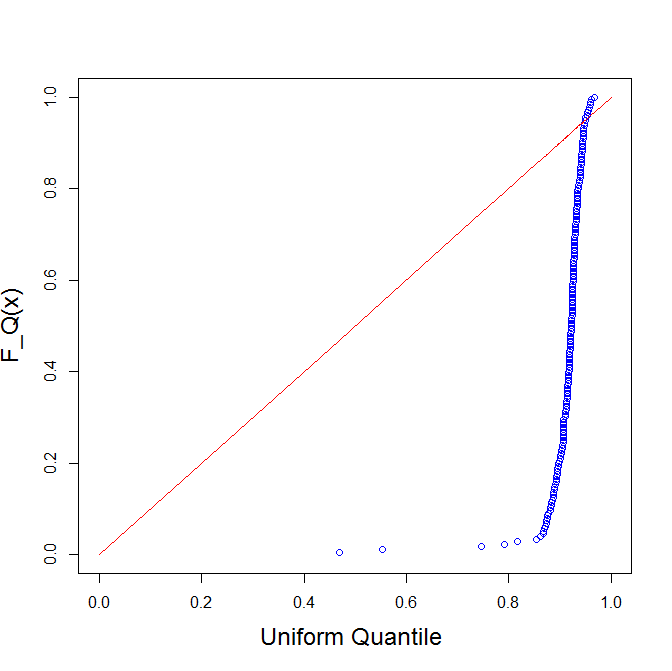
\includegraphics[width=.45\linewidth]{CDF_1w_Real.png}}
\hfill
\subfigure[2w Horizon]{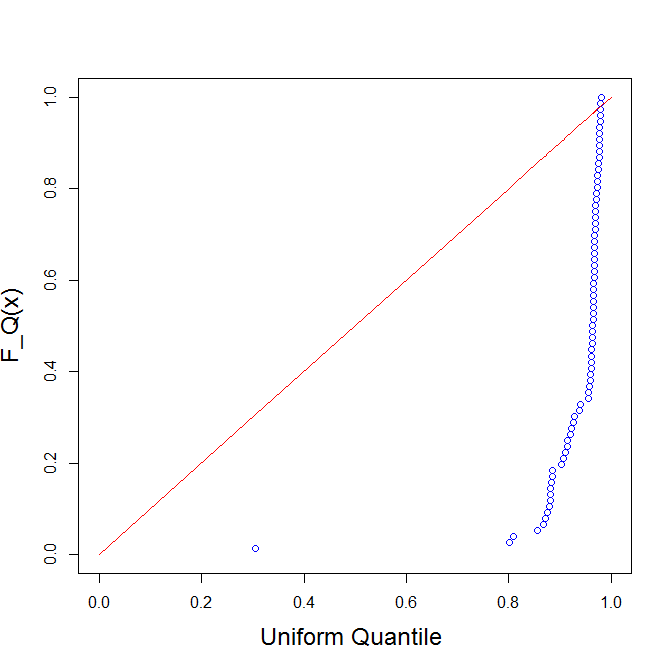
\includegraphics[width=.45\linewidth]{CDF_2w_Real.png}}
\caption{Quantile distribution $F_{Q}$ (blue dots) against standard uniform distribution $U$ (red line) using real market scenarios. We have $F_{Q}$ mostly inferior to $U$ except towards the upper-right edge of the plot.} 
\label{fig:FirstOrderTestResults}
\end{figure}

\begin{figure}[h] 
\hfill
\subfigure[Hypothetical Market Scenario]{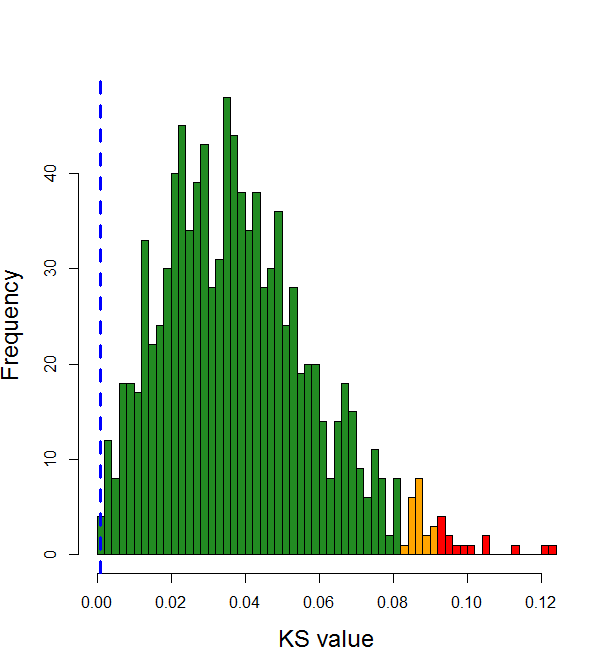
\includegraphics[width=.45\linewidth]{KS_1W_hypo.png}}
\hfill
\subfigure[Real Market Scenario]{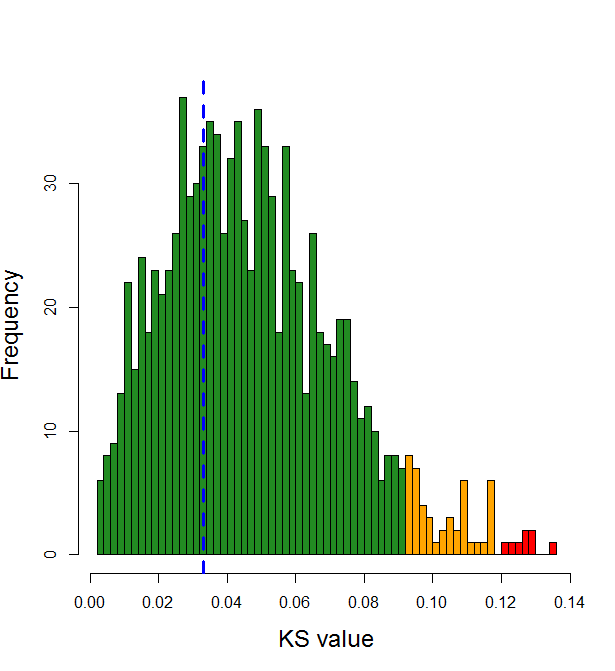
\includegraphics[width=.45\linewidth]{KS_1W_real.png}}
\hfill
\caption{Historical backtesting results with forecasting horizon of 1w, with the one-sided $D^+$ metric("KS value"). The blue dot-line is $D^{\textrm{Model}}$ and the histogram is based on $\{D^{\textrm{ideal}}_j\}_{j=1}^K$ values. With the Hypothetical Market Scenarios, $D^{\textrm{Model}}$ = 0.001 (0.10 p-value) while with the Real Market Scenarios, $D^{\textrm{Model}}$ = 0.033 (31.27 p-value).}
\label{fig:backtestingHistogram1w}
\end{figure}

\begin{figure}[!h] 
\hfill
\subfigure[Hypothetical Market Scenario]{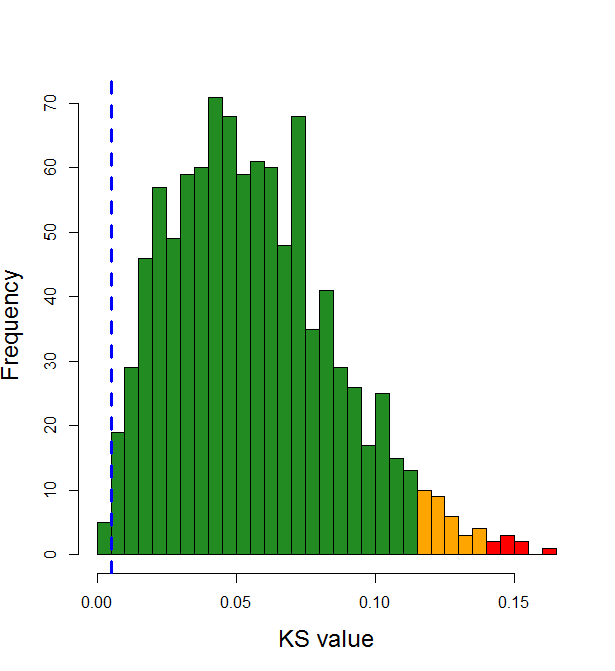
\includegraphics[width=.45\linewidth]{KS_2W_hypo.png}}
\hfill
\subfigure[Real Market Scenario]{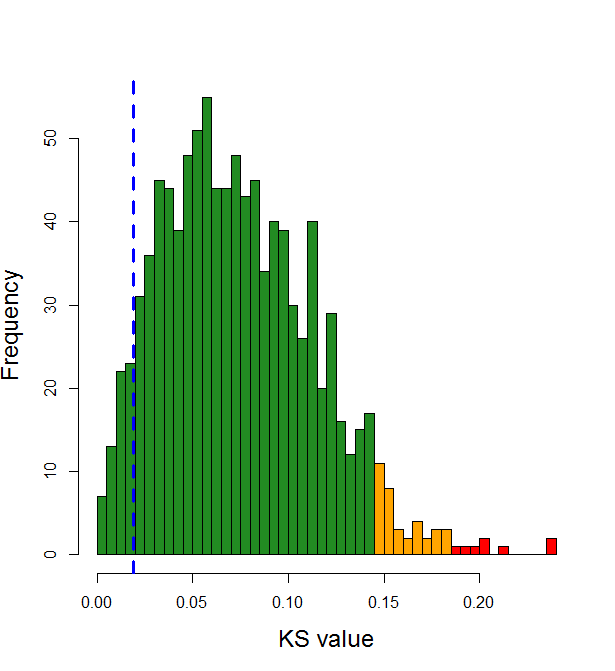
\includegraphics[width=.45\linewidth]{KS_2W_real.png}}
\hfill
\caption{Historical backtesting results with forecasting horizon of 2w, with the one-sided $D^+$ metric("KS value"). The blue dot-line is $D^{\textrm{Model}}$ and the histogram is based on $\{D^{\textrm{ideal}}_j\}_{j=1}^K$ values. With the Hypothetical Market Scenarios, $D^{\textrm{Model}}$ = 0.005 (0.40 p-value) while with the Real Market Scenarios, $D^{\textrm{Model}}$ = 0.019 (5.50 p-value).}
\label{fig:backtestingHistogram2w}
\end{figure}

Another approach to assess the appropriateness of the model is with respect to a given definition of $D$-metric. There are many appropriate choices, but for simplicity, we demonstrate with the Kolmogorov-Smirnov statistic \cite{kolmogorov1933}, where the distance $D$ between the distribution of percentile  $F_{\textrm{Q}}(x)$ and the standard uniform $U(x)$ is defined as:
\begin{equation}
D=\sup_{x\in [0,1] }|F_{\textrm{Q}}(x)-U(x)|
\end{equation}

This distance metric is \emph{two-sided} in the sense that what we test is how much the model distribution fits the data observed. As we noticed already in Figure \ref{fig:FirstOrderTestResults}, we already know that our simulated IM distribution is not accurate with respect to the historical IM distribution. Instead, we aim to demonstrate that our simulated IM distribution sufficiently underestimates that of the historical IM distribution. To this end, we instead define a \emph{one-sided} metric $D^{+}$:
\begin{equation}
D^+=\sup_{x \in [0,1]}(F_{\textrm{Q}}(x)-U(x))
\end{equation}
to test whether the IM amounts simulated are consistently underestimated in comparison to historical SIMM amounts.  

We use this one-sided Kolmogorov-Smirnov metric for our historical backtesting test. Follow the procedure outlined in Section \ref{s:BacktestingProcedure}, we plot the distance $D^{\textrm{Model}}$ against the histogram of $\{D^{\textrm{ideal}}_j\}_{j=1}^K$ in Figures \ref{fig:backtestingHistogram1w}, \ref{fig:backtestingHistogram2w}. The blue dot-line represents the $D^{\textrm{Model}}$ value. Further, to define a confidence interval for the $D^{\textrm{Model}}$ value, as will as to provide a \emph{traffic-light} system for model risk monitoring, we use similar the same band coding colour suggested in \cite{ruiz2014backtesting}:

\begin{itemize}
\item Green: the band 0-95 percent of the first $D^{\textrm{ideal}}$ values
\item Orange: the band 95-99 percent of the first $D^{\textrm{ideal}}$ values
\item Red: the band 99-100 percent of the first $D^{\textrm{ideal}}$ values
\end{itemize}

From Figures \ref{fig:backtestingHistogram1w}, \ref{fig:backtestingHistogram2w}, we observe that the $D^{\textrm{Model}}$ values are comfortably in the green band confidence interval in either the Hypothetical Market Scenario or the Real Market Scenario. This suggests that the simulated IM distribution conservatively underestimates the historical IM distribution, with respect to the one-sided Kolmogorov-Smirnov metric. 

\section{Conclusions} \label{sec:conclusion}

In this paper, we propose simple approximation approaches to forward simulate bilateral initial margin requirements. These approaches are not only practical to implement in realistic production environments, but are also conservative under the context of counterparty credit risk management and regulatory capital calculation.

In conjunction, we also propose a series of testing approaches to assess the model appropriateness in terms of both model's in-simulation consistency and historical backtesting. Further, these testing approaches are not specific to our initial margin simulation methodology, and should be applicable to a broad class of initial margin simulation approaches.

\clearpage

\section*{Reference}
\bibliographystyle{model1-num-names}
\bibliography{ref.bib}

\end{document}
